\graphicspath{{figures/modeling/gearTrain/}}
\section{Modeling of the Gear System}\label{sec:ModGearSys}
This section aims to describe the behaviour of the gear system and the transfer functions that needs to be found are shown on 
\autoref{fig:GearSystemDiagram}.
Two transfer functions are going to be determined in this section: The relation between the motor velocity, $\omega_m$, and the angle of the arm, $\theta_a$, and the load torque,$\tau_l$, generated by the gears.
\begin{figure}[htbp]
	\centering
	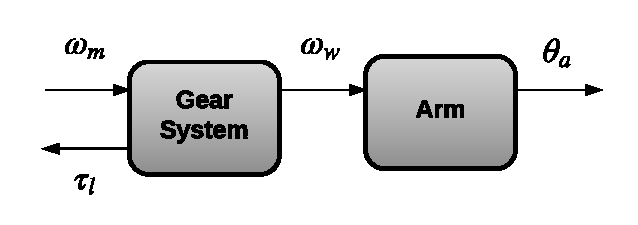
\includegraphics[width=0.6\textwidth]{InputOutputGear}
	\caption{Block diagram of the inputs and outputs of the gear system.}
	\label{fig:GearSystemDiagram}
\end{figure}
\startexplain
\explain{$\tau_l$ is the torque of the motor's load}{\si{\newton\meter}}
\explain{$\omega_m$ is the motor's angular velocity}{\si{\meter\per\second}}
\explain{$\tau_{as}$ is the torque of the arm and the stick}{\si{\newton\meter}}
\explain{$\omega_{w_3}$ is the third wheel's angular velocity}{\si{\meter\per\second}}
\stopexplain


\subsection{Relation between Motor Velocity and Angle of the Arm}
The motor is connected to the first wheel of the gear system by a belt as shown on \autoref{fig:Belt&Pulley}. The first wheel has a smaller wheel rigidly attached and turning in the same direction. The smaller first wheel is attached to the second wheel in the same fashion as the motor to the first wheel. Wheel two and three are exactly the same as wheel one and two. The entire system can thus be described \autoref{fig:Belt&Pulley} by replacing the motor wheel with the smaller wheels 1 and 2 and the larger wheel 1 with the larger wheels 2 and 3.

\begin{figure}[htbp]
	\centering
	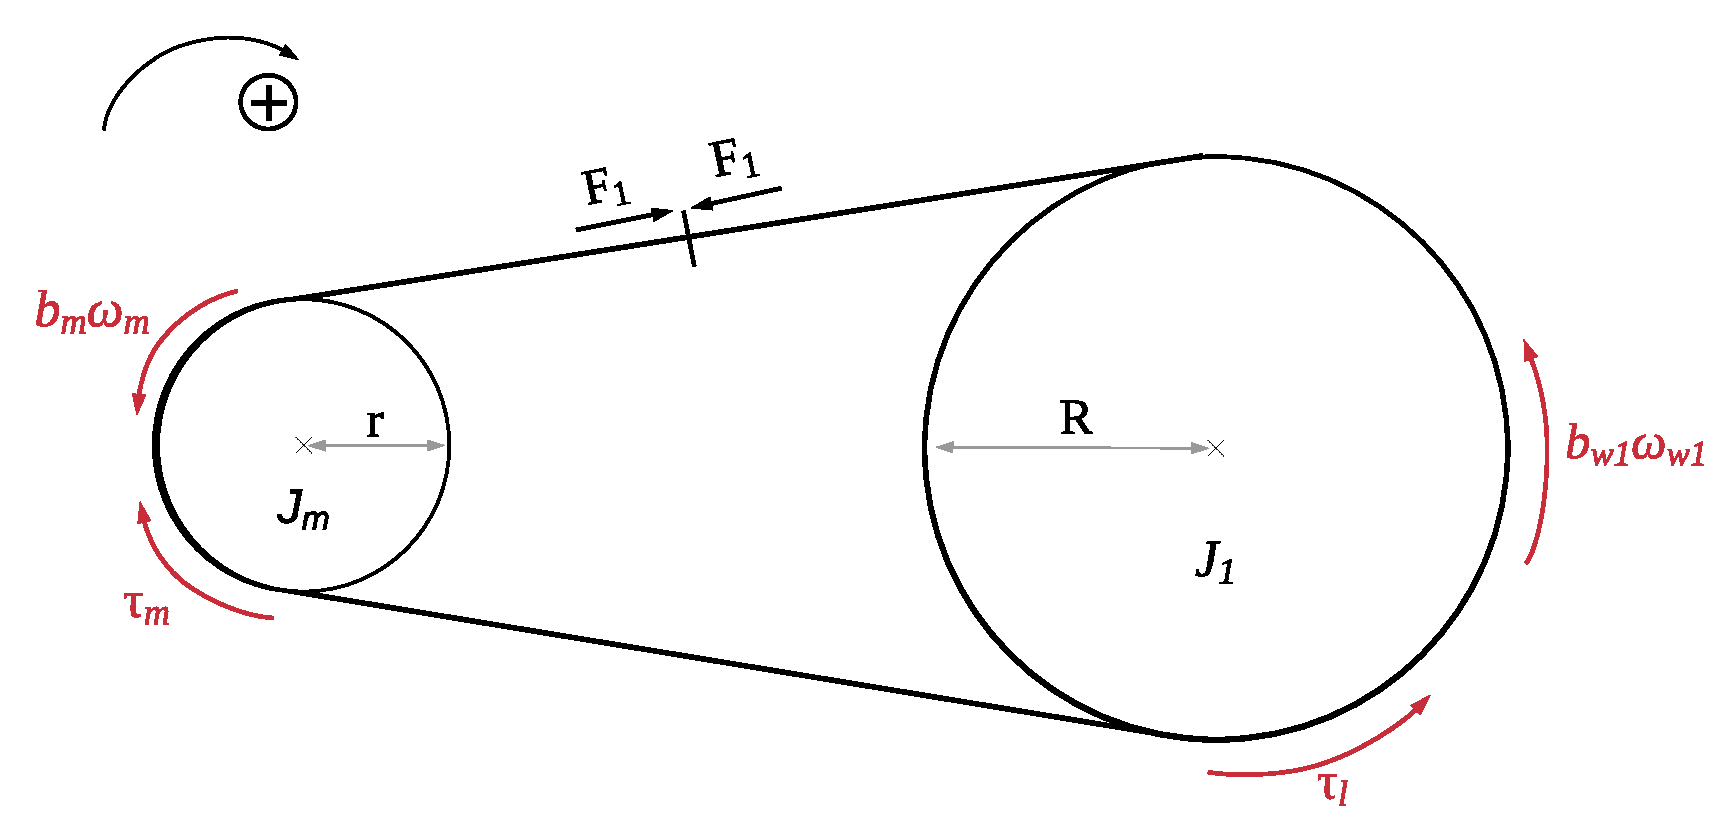
\includegraphics[width=0.9\textwidth]{figures/modeling/gearTrain/GearAndBeltSystem.pdf}
	\caption{Free body diagram of the motor wheel system.}
	\label{fig:Belt&Pulley}
\end{figure}
\startexplain
\explain{$J_m$ is the moment of inertia of the motor}{\si{\kilogram\meter\squared}}
\explain{$J_w$ is the moment of inertia of the wheel}{\si{\kilogram\meter\squared}}
\explain{$\omega_m$ is the motor's angular velocity}{\si{\meter\per\second}}
\explain{$\tau_m$ is the torque of the motor}{\si{\newton\meter}}
\explain{$F_1$ is the force transferred from the motor to the wheel}{\si{\newton}}
\explain{$r$ is the radius of the motor's wheel}{\si{\meter}}
\explain{$R$ is the radius of the wheel}{\si{\meter}}
\explain{$\tau_f$ is the torque of the gear train friction}{\si{\newton\meter}}
\explain{$\tau_L$ is the torque of the wheel's load}{\si{\newton\meter}}
\explain{$b_w$ is the viscous friction coefficient of the wheel}{\si{\newton\meter\second}}
\stopexplain

If the motor shaft turns, the belt joining the small and the big wheel will make them turn the same distance, giving relation in \autoref{eq:motorWheelDistance}.
\begin{flalign}
	\theta_m r = \theta_w R \label{eq:motorWheelDistance}
\end{flalign}

This expression is then differentiated to find the relation with the angular velocities in \autoref{eq:AngularVelRelation}.
\begin{flalign}
	\omega_m r = \omega_w R
	\label{eq:AngularVelRelation}
\end{flalign}

The gear ratio can then be defined by \autoref{eq:GearRatio}.
\begin{flalign}
	N = \frac{r}{R} \label{eq:GearRatio}
\end{flalign}

As the gear system is composed by three similar connected wheels structures like \autoref{fig:Belt&Pulley}, the ratio between one of the small wheels, $r_x$, and the big wheel connected by the belt, $R_x$ is the same and is seen in \autoref{eq:GearRatioForAll}.
\begin{flalign}
	\frac{r_x}{R_x} = \frac{r_{motor}}{R_{w_1}} = \frac{r_{w_1}}{R_{w_2}} = \frac{r_{w_2}}{R_{w_3}} = N \label{eq:GearRatioForAll}
\end{flalign}

Knowing this and since $\omega_m$ is transferred through three gears reductions, the relation between the angular velocity of the motor $\omega_m$ and the angle of the arm $\theta_a$ is found following the principle of \autoref{eq:AngularVelRelation}.
\begin{subequations} \label{eq:tech_ToA}
	\begin{flalign}
		&\omega_a(t) = N^3 \omega_m(t) \\
		&\theta_a(t) = N^3 \int_{0}^{t}\omega_m(v) dv \\
		&\mathcal{L}\{\theta_a(t)\} = \Theta_a(s) = N^3 \cdot \frac{1}{s} \Omega_m(s) 
	\end{flalign}
\end{subequations}

The transfer function from the motor's angle velocity to the angle of the arm becomes \autoref{eq:thetaOmega}.
\begin{equation}\label{eq:thetaOmega}
	\frac{\Theta_a(s)}{\Omega_m(s)} =  \frac{N^3}{s}
\end{equation}

\subsection{Determining the Load Torque Produced by the Gears}\label{sec:torqueGear}
The torque of the load put on the motor is the sum of the torque produced by the gears and the torque produced by the arm and stick. As the torque from the arm and stick are considered negligible c.f. \autoref{sec:StickArm}, only the torque of the gears needs to be described.

%Now that the relationship between $\theta_a$ and $\omega_m$ is found, $\tau_l$ is studied. In the inverted pendulum case the load is composed of the friction and the torque necessary to counter the gravity and the momentums which result in \autoref{eq:TauL}.
%
%\begin{equation}\label{eq:TauL}
%	\tau_l = \tau_{gear} + \tau_{as} \addunit{\newton\meter}
%\end{equation}
%\startexplain
%\explain{$\tau_{gear}$ is the load from the gear system}{\si{\newton\meter}}
%\explain{$\tau_{as}$ is the load from the arm and the stick}{\si{\newton\meter}}
%\stopexplain


%\subsubsection*{Determining $\tau_{gear}$}
%The gear train is composed by three identical belt and pulley system. \autoref{fig:Belt&Pulley} corresponds to the first system between the motor and the first wheel. 

%Using the previously stated $2^{nd}$ law of motion, the mechanical equation for the motor wheel can be found from \autoref{fig:MotorBodyDiagram}:
The torque on the wheel of the motor can be described by \autoref{eq:MotorfreeBody}.
\begin{flalign}
J_{m} \dot{\omega}_{m} &= \tau_{m} - \tau_{l} - \tau_{fm} \\
J_m \dot{\omega}_m &= \tau_m + F_1r - b_m\omega_m \label{eq:MotorfreeBody}
\end{flalign}

This means that the torque of the load produced by the gears is equal to $-F_1r$. To find $F_1$ the torque on the wheel is examined and seen in \autoref{eq:TauW1}.
\begin{flalign}
	J_w\dot{\omega}_{w} = -F_1R -\tau_L -b_{w}\omega_{w} \label{eq:TauW1}
\end{flalign}

Here $\tau_L$ is the load on wheel 1 that comes from the rest of the wheels connected to it. Wheel 2 is connected to wheel 1 similar to how wheel 1 is connected to the motor. This means that the load torque on wheel 1 is related to $F_2$ and the load torque on wheel 2 is related to $F_3$. Substituting the load torque for the forces, the torques for each wheel is \autoref{eq:GiveMeAnOriginalName}.
\begin{subequations}\label{eq:GiveMeAnOriginalName} 
	\begin{flalign} 
		&J_{w_1}\dot{\omega}_{w_1} = -F_1R + F_2r -b_{w_1}\omega_{w_1} \\ 
		&J_{w_2}\dot{\omega}_{w_2} = -F_2R + F_3r -b_{w_2}\omega_{w_2} \\ 
		&J_{w_3}\dot{\omega}_{w_3} = -F_3R - b_{w_3}\omega_{w_3} 
	\end{flalign}
\end{subequations}

Using the relation in \autoref{eq:AngularVelRelation}, the angular velocity of each wheels can be found to be \autoref{eq:WheelAngularVelocity}.
\begin{subequations} \label{eq:WheelAngularVelocity}
	\begin{flalign}
		&\omega_{w_1} = N \omega_m \\
		&\omega_{w_2} = N \omega_{w_1} = N^2 \omega_m \\
		&\omega_{w_3} = N \omega_{w_2} = N^3 \omega_m 
	\end{flalign}
\end{subequations}

The same equations are valid with angular accelerations and are inserted in \autoref{eq:GiveMeAnOriginalName} giving \autoref{eq:TauWheelRelation}.
\begin{subequations} \label{eq:TauWheelRelation}
	\begin{flalign}  
		&J_{w_1}N\dot{\omega}_m = -F_1R + F_2r -b_{w_1}N\omega_m \\ 
		&J_{w_2}N^2\dot{\omega}_m = -F_2R + F_3r -b_{w_2}N^2\omega_m  \\ 
		&J_{w_3}N^3\dot{\omega}_m = -F_3R - b_{w_3}N^3\omega_m  
	\end{flalign}
\end{subequations}

%In order to simplify the frictions, they are considered to be wet friction as such the frictions in the gear system are directly dependent on the angular velocity of the wheels. When the system is not moving:
%\begin{subequations} 
%	\begin{flalign}  \label{eq:TaufTgearConditions}
%	\tau_L &= \tau_{gear}\\
%	\omega_m &= 0
%	\end{flalign}
%\end{subequations}
%
%Inserting \autoref{eq:TaufTgearConditions} into \autoref{eq:MotorfreeBody}:
%\begin{equation} 
%		\tau_{gear} = -F_1 \cdot r \addunit{\newton\meter}
%		\label{eq:TaufF1r}
%\end{equation}

The forces $F_1$, $F_2$ and $F_3$ are isolated giving \autoref{eq:F1F2F3}.

\begin{subequations} \label{eq:F1F2F3}
	\begin{flalign}
		&F_1 = -\frac{1}{R} N\left(b_{w_1}\omega_m + J_{w_1}\dot{\omega}_m - \frac{F_2r}{N}\right) \label{eq:F1} \\ 
		&F_2 = -\frac{1}{R} N^2\left(b_{w_2}\omega_m + J_{w_2}\dot{\omega}_m - \frac{F_3r}{N^2}\right) \label{eq:F2} \\
		&F_3 = -\frac{1}{R} N^3\left(b_{w_3}\omega_m + J_{w_3}\dot{\omega}_m\right) \label{eq:F3}
	\end{flalign}
\end{subequations}

Inserting \autoref{eq:F3} in \autoref{eq:F2} gives \autoref{eq:F3F2}.

\begin{flalign}
F_2=-\frac{1}{R}N^2\left(b_{w_2}\omega_m + J_{w_2}\dot{\omega}_m +\frac{r}{R}\frac{N^3}{N^2}\left(b_{w_3}\omega_m + J_{w_3}\dot{\omega}_m\right)\right) \label{eq:F3F2}
\end{flalign}

\autoref{eq:F3F2} is then inserted in \autoref{eq:F1} giving \autoref{eq:F3F2F1} while remembering that the gear ratio is defined by \autoref{eq:GearRatio}.
\begin{flalign}
F_1 = -&\frac{1}{R}N\Big(b_{w_1}\omega_m + J_{w_1}\dot{\omega}_m \notag \\
+&N^2\big(b_{w_2}\omega_m + J_{w_2}\dot{\omega}_m \notag \\ 
+&N^2\left(b_{w_3}\omega_m + J_{w_3}\dot{\omega}_m\right)\big)\Big) \label{eq:F3F2F1}
\end{flalign}

Since $\tau_l=-F_1r$ and the torque of the load on the motor is the torque of the gears, $\tau_{gear}$ can be expressed by \autoref{eq:TaufTimeDomain}.
\begin{flalign} 
\tau_{gear} = N^2 & \Big(b_{w_1}\omega_m + J_{w_1}\dot{\omega}_m \notag \\
+N^2 & \big(b_{w_2}\omega_m + J_{w_2}\dot{\omega}_m \notag \\
+N^2 &(b_{w_3}\omega_m + J_{w_3}\dot{\omega}_m)\big)\Big) \label{eq:TaufTimeDomain}
\end{flalign}

\autoref{eq:TaufTimeDomain} is Laplace-transformed and reorganized giving \autoref{eq:TaufReorganized}.
\begin{subequations}
\begin{flalign}
\mathcal{L}\{\tau_{gear}(t)\} = \tau_{gear}(s) = N^2 & \Big(B_{w_1}\Omega_m + sJ_{w_1}\Omega_m \notag \\
+N^2 & \big(B_{w_2}\Omega_m + sJ_{w_2}\Omega_m \notag \\
+N^2 & (B_{w_3}\Omega_m + sJ_{w_3}\Omega_m)\big)\Big) \label{eq:TaufLaplaceDomain} \\
\tau_{gear} = \Big(\big(N^2 J_{w_1} + N^4 J_{w_2} + N^6 J_{w_3})s + &\big( N^2 B_{w_1} + N^4 B_{w_2} + N^6 B_{w_3}\big)\Big)\Omega_m \label{eq:TaufReorganized}
\end{flalign}
\end{subequations}

The moments of inertia and the frictions for each wheel is grouped into two variables $J_{gear}$ and $B_{gear}$ respectively giving the torque for the gears in \autoref{eq:TaufSimplified}.
\begin{flalign}
\tau_{gear} = \left(J_{gear}s +B_{gear}\right)\Omega_m 	\label{eq:TaufSimplified}
\end{flalign}











%\subsubsection*{Determining $\tau_{as}$}
%
%$\tau_{as}$ is the torque necessary for the motor to counter the load applied by the arm and the stick. It can be divided into two parts as in \autoref{eq:TauasBegin}.
%
%\begin{equation}\label{eq:TauasBegin}
%	\tau_{as}=\tau_a+\tau_s \addunit{\newton\meter}
%\end{equation}
%\startexplain
%\explain{$\tau_a$ is the load of the arm}{\si{\newton\meter}}
%\explain{$\tau_s$ is the load of the stick}{\si{\newton\meter}}
%\stopexplain
%
%The first part is the torque to counter the load of the arm, $\tau_a$.
% 
% \begin{figure}[htbp]
% 	\centering
% 	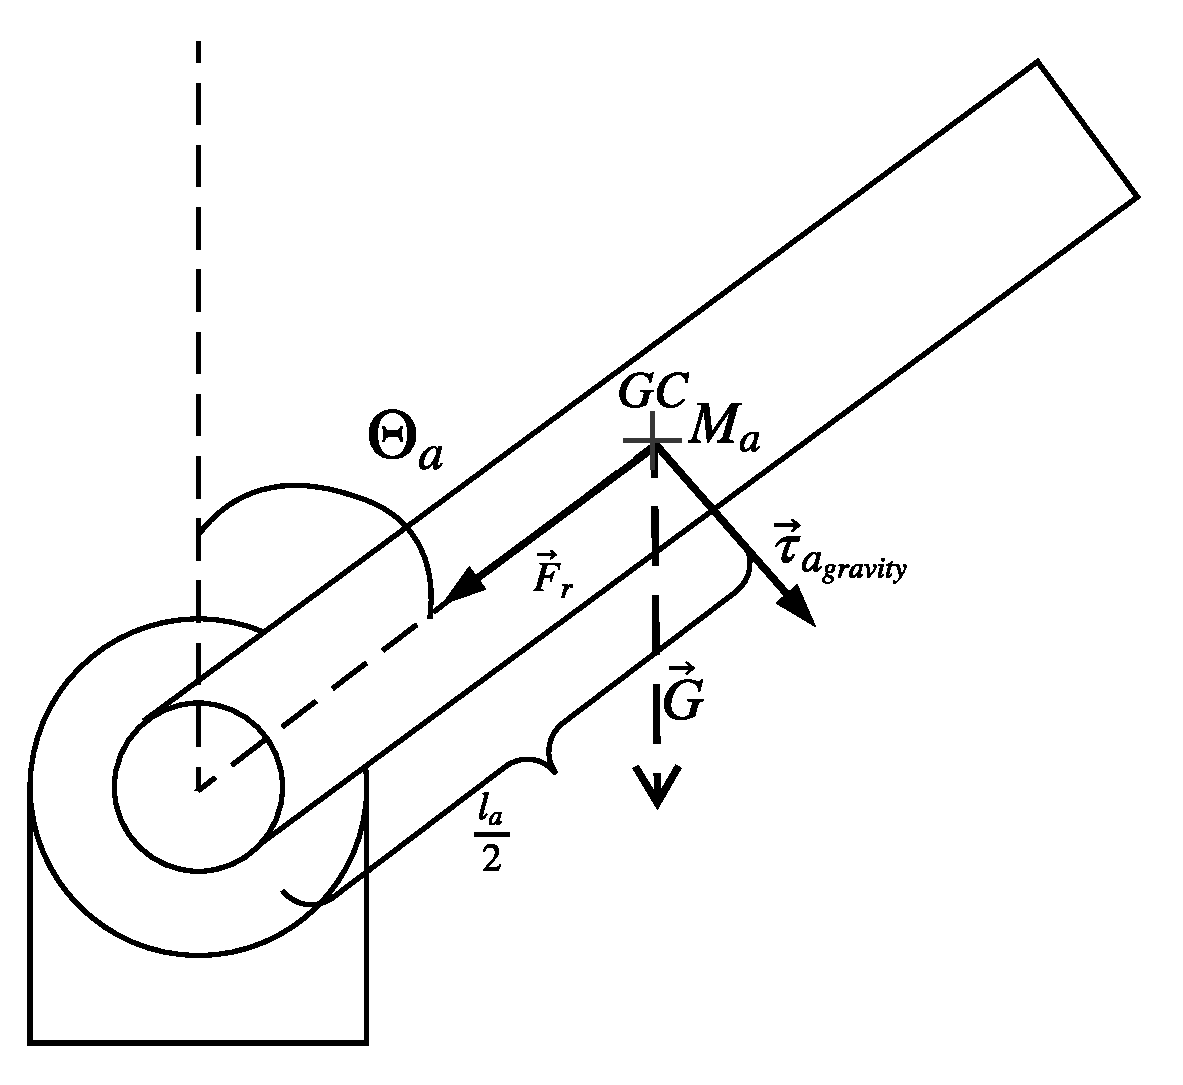
\includegraphics[width=0.5\textwidth]{PendulumWithWeightlessRod}
% 	\caption{Approximation of the arm as a weightless rod pendulum}\label{fig:tauAgrav}
% \end{figure}
% \startexplain
% \explain{$\vec{G}$ is the gravity force}{\si{\kilogram\meter\per\second\squared}}
% \explain{$\vec{F}_r$ is the reaction force of the arm to the gravity}{\si{\kilogram\meter\per\second\squared}}
% \explain{$\tau_{a_{gravity}}$ is the torque remaining of the gravity after substracting $\vec{F}_r$}{\si{\newton\meter}}
% \explain{$l_a$ is the length of the arm}{\si{\meter}}
% \stopexplain
% 
%According to \autoref{fig:tauAgrav}, the $2^{nd}$ and the $3^{rd}$ Newton's law \autoref{eq:tauA} can be deduced.
%
%\begin{equation}\label{eq:tauA}
%	J_a \ddot{\theta}_a=\vec{G}_a-\tau_a \addunit{\newton\meter}
%\end{equation}
%\startexplain
%\explain{$M_a$ is the mass of the arm}{\si{\kilogram}}
%\explain{$\tau_a$ is the reaction torque from the motor}{\si{\newton\meter}}
%\explain{$J_a$ is the moment of inertia of the arm}{\si{\kilogram\meter\squared}}
%\stopexplain
%
%By assuming the arm to be a pendulum with a weightless rod and by geometry law \autoref{eq:tauA} can be derived into \autoref{eq:tauARot}
%
%\begin{equation}\label{eq:tauARot}
%	\tau_a=-J_a\ddot{\theta}_a+\frac{l_a}{2}M_a g sin(\theta_a) \addunit{\newton\meter}
%\end{equation}
%
%By linearizing \autoref{eq:tauA}, \autoref{eq:finalTauA} is derived.
%
%\begin{flalign}\label{eq:finalTauA}
%	\tau_a&=-J_a \ddot{\theta}_a+M_a g \frac{l_a}{2} \theta_a \addunit{\newton\meter} \notag\\
%	\mathcal{L}\{\tau_a\}=\tau_a(s)&=-J_a\Theta_a s^2+M_a g \frac{l_a}{2} \Theta_a \addunit{1}
%\end{flalign}
%
%Now, the load of the stick $\tau_s$ is studied. Unlike the arm, it is not directly connected to the gear train, so it  has to be defined in a new base in order to be used with the arm. The Fresnel base has $\tau_s$ is on one of the axis as seen in \autoref{fig:loadStick}.
%
% \begin{figure}[htbp]
% 	\centering
% 	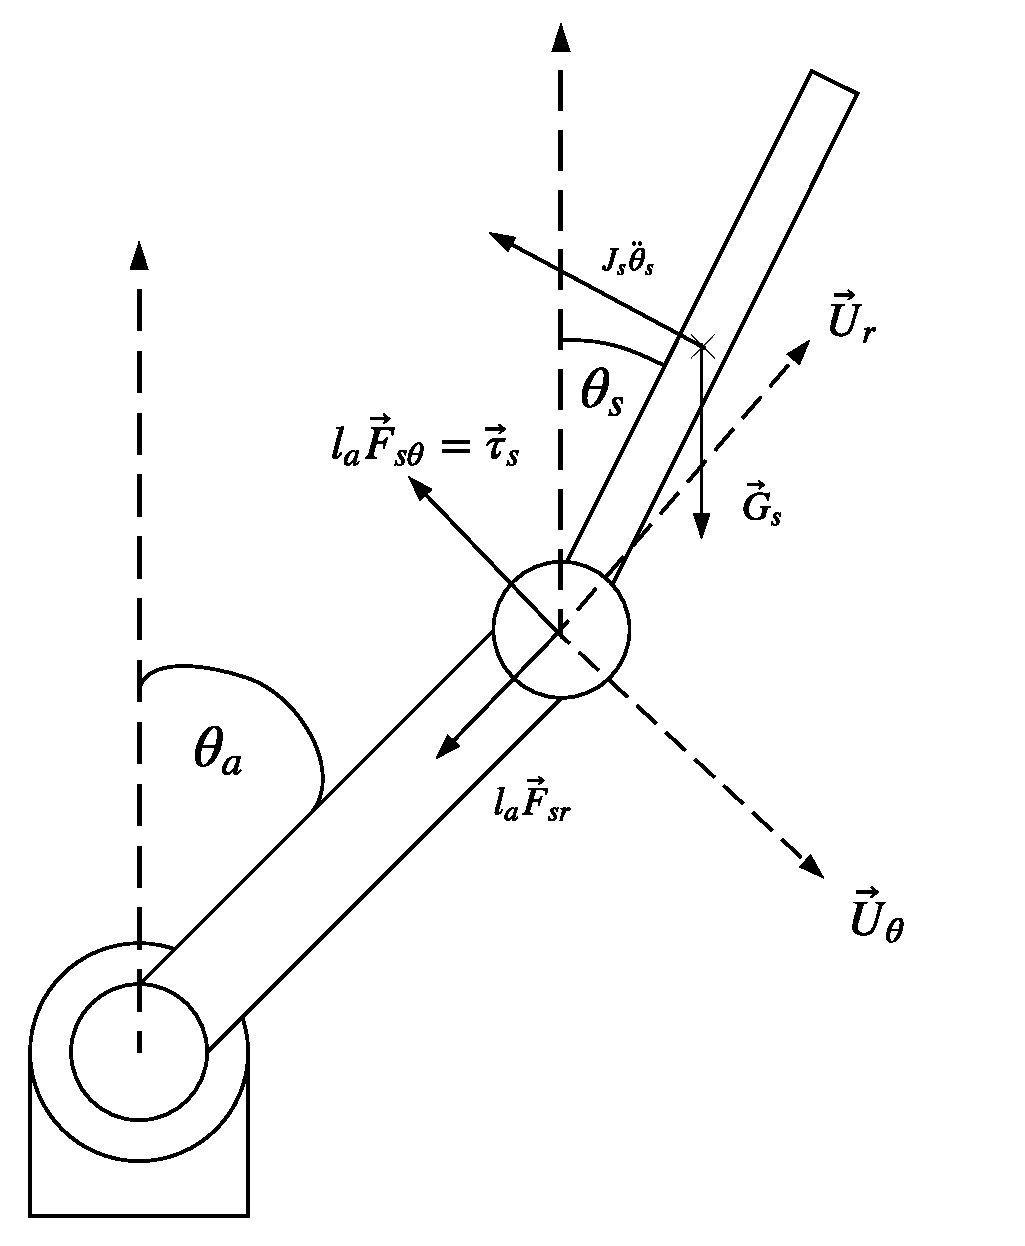
\includegraphics[width=0.5\textwidth]{loadOnThetaA}
% 	\caption{Load applied by the stick translated in the Fresnel base}\label{fig:loadStick}
% \end{figure}
% \startexplain
% \explain{$\vec{G}_s$ is the gravity force applied on the stick}{\si{\kilogram\meter\per\second\squared}}
% \explain{$\vec{F}_{sr}$ is the reaction force of the arm to the load of the stick}{\si{\kilogram\meter\per\second\squared}}
% \explain{$\vec{F}_{s\theta}$ is the force generated by the stick}{\si{\kilogram\meter\per\second\squared}}
% \explain{$\tau_{s}$ is the load applied by the stick on the gear train}{\si{\newton\meter}}
% \explain{$l_a$ is the length of the arm}{\si{\meter}}
% \stopexplain
%
%This gives, by Newton's $2^{nd}$ law, \autoref{eq:tauSBase}
%
%\begin{subequations}\label{eq:tauSBase}
%	\begin{flalign}
%		J_s\vec{\ddot{\theta}}_{s\theta}&=\vec{G}_{s\theta}+\vec{F}_{s\theta} \addunit{\newton\meter}\\
%		J_s\vec{\ddot{\theta}}_{sr}&=\vec{G}_{sr}+\vec{F}_{sr} \addunit{\newton\meter} \addunit{\newton\meter}
%	\end{flalign}
%\end{subequations}
%
%As said in \autoref{fig:loadStick}, $\vec{F}_{sr}$ is the reaction force from the arm, and since it is assumed that the arm is incompressible, this force is cancelled. This leaves only a dependency on $\vec{U}_{\theta}$, which, by applying geometric properties, gives \autoref{eq:Fso}.
%
%\begin{flalign}\label{eq:Fso}
%	-cos(\theta_a-\theta_s)J_s\ddot{\theta}_s&=-M_sg\left(l_asin(\theta_a)+\frac{l_s}{2}sin(\theta_s)\right)cos(\theta_a) \notag\\
%	&+l_aF_{s\theta} \addunit{\newton\meter}
%\end{flalign}
%
%\autoref{eq:Fso} combined with Newton $3^{rd}$ law gives $\tau_s$ as explained in \autoref{eq:tauS}.
%
%\begin{subequations}\label{eq:tauS}
%	\begin{flalign}
%		\tau_s&=l_aF_{s\theta} \addunit{\newton\meter}\\
%		\tau_s&=-cos(\theta_a-\theta_s)J_s\ddot{\theta}_s+M_sg\left(l_asin(\theta_a)+\frac{l_s}{2}sin(\theta_s)\right)cos(\theta_a)\addunit{\newton\meter}
%	\end{flalign}
%\end{subequations}
%
%By linearizing \autoref{eq:tauS}, \autoref{eq:LinTauS} is found.
%
%\begin{flalign}\label{eq:LinTauS}
%	\tau_s = -J_s \ddot{\theta_s} s^2 + M_s g \left(\theta_a l_a+\frac{l_s}{2}\theta_s\right) \addunit{\newton\meter}    
%\end{flalign}
%
%When controlling the equilibrium of the stick, $\theta_s$ grows up to only a couple degrees, not exceeding 10. Therefore, regarding the torque generated by the stick, $\theta_s$ can be considered as 0. Thus giving:
%
%\begin{equation}\label{eq:FinalTauS}
%	\mathcal{L}\{\tau_{s}\}=\tau_{s}(s)=M_sgl_a\Theta_a \addunit{1}
%\end{equation}
%
%
%
%At last $\tau_{as}$ is found by combining Equations \eqref{eq:finalTauA} and \eqref{eq:FinalTauS} in \autoref{eq:FinalTauAS}.
%
%\begin{subequations}\label{eq:FinalTauAS}
%	\begin{flalign}
%		\tau_{as} &=\tau_a+\tau_s \addunit{\newton\meter}\\
%		&= -J_a\Theta_a s^2+M_a g \frac{l_a}{2} \Theta_a+M_sgl_a\Theta_a  \addunit{1}
%	\end{flalign}
%\end{subequations} 
%
%By combining Equations \eqref{eq:TauL}, \eqref{eq:FinalTauAS} and \eqref{eq:TaufSimplified}, $\tau_l$ is then defined as \autoref{eq:finalTauL}.
%
%\begin{equation}\label{eq:finalTauL}
%	\tau_l=M_ag\frac{l_a}{2}\Theta_a-J_a\Theta_a s^2+M_sgl_a\Theta_a +(J_{gear}s +B_{gear})\Omega_m(s)
%\end{equation}
%
%Now that $\tau_l$ is found, it is re-injected in \autoref{eq:Iinserted} giving \autoref{eq:begTFOaUm}.
%
%\begin{align}\label{eq:begTFOaUm}
%s J_{m} \Omega_m(s) &=K_{t} \frac{U_m-K_e \Omega_m(s)}{R_m} - \Big(M_ag\frac{l_a}{2}\Theta_a-J_a\Theta_a s^2 +M_sgl_a\Theta_a \notag \\ 
%&+ (J_{gear}s +B_{gear})\Omega_m(s)\Big) - B_{m} \Omega_m(s) 
%\end{align}
%
%$\Omega_m(s)$ is expressed according to $\Theta_a$ with \autoref{eq:thetaOmega}.
%
%\begin{flalign}\label{eq:begTFOaUm2}
%\frac{J_{m}}{N^3}\Theta_a s^2 &=K_{t} \frac{U_m-K_e \frac{s}{N^3}\Theta_a}{R_m}- \Big(M_ag\frac{l_a}{2}\Theta_a-J_a\Theta_as^2 +M_sgl_a\Theta_a   \notag \\ 
%&+ (J_{gear}s +B_{gear})\frac{s}{N^3}\Theta_a\Big) - B_{m} \frac{s}{N^3}\Theta_a 
%\end{flalign}
%
%
%Factorizing \autoref{eq:begTFOaUm2} by $\Theta_a$ and $U_m$, \autoref{eq:midTFOaUm} is obtained.
%
%\begin{flalign}\label{eq:midTFOaUm}
%\frac{K_t}{R_m}U_m	&= \Theta_a\Big[ \frac{J_{m}}{N^3}s^2 + \frac{K_e K_t}{R_mN^3}s + M_ag\frac{l_a}{2} - J_a s^2 + M_sgl_a \notag \\
%					&+ \frac{J_{gear}}{N^3}s^2+\frac{B_{gear}}{N^3}s + \frac{B_{m}}{N^3}s \Big]
%\end{flalign}
%
%\autoref{eq:midTFOaUm} is then organized to find $\nicefrac{\Theta_a}{U_m}$.
%\begin{flalign}\label{eq:UmThetaaTFSimplified}
%\frac{\Theta_a}{U_m}&= \frac{\nicefrac{K_t}{R_m}}{\left( \frac{J_{m}+J_{gear}}{N^3} - J_a \right)s^2 + \left( \nicefrac{\left( \frac{K_e K_t}{R_m} + B_{gear} + B_{m}\right)}{N^3} \right) s + gl_a(M_s+M_a)}
%\end{flalign}

%
%
%
%
%

Now that $\tau_l$ is found, it is re-injected in \autoref{eq:Iinserted} giving \autoref{eq:UmtoThetaa1}. 
\begin{flalign}\label{eq:UmtoThetaa1}
	s\cdot J_m\cdot \Omega_m(s) & =K_t\frac{U_m(s)-K_e\cdot \Omega_m(s)}{R_m+sL_m}-\big(-J_a\Theta_a s^2+M_ag\frac{l_a}{2}\Theta_a \notag \\ 
	& +M_sl_a\Theta_a+s^2\frac{l_s}{2}l_aM_s\Theta_a+s^2\frac{l_s^2}{4}M_s\left(\frac{\frac{-3l_a}{2l_s}s^2}{s^2-\frac{3g}{2l_s}}\right)\Theta_a \notag\\
	& +(J_{gear}s +B_{gear})\Omega_m(s) \big) - B_m \cdot \Omega_m(s)
\end{flalign}

$\Omega_m(s)$ is expressed according to $\Theta_a$ with \autoref{eq:thetaOmega}. 
\begin{flalign}\label{eq:UmtoThetaa2}
	s\cdot J_{m}\cdot \frac{s}{N^3}\Theta_a &=K_{t}\frac{U_m(s)-K_e\cdot \frac{s}{N^3}\Theta_a}{R_m+sL_m}-\Big( -J_a\Theta_a s^2+M_ag\frac{l_a}{2}\Theta_a \notag\\ 
	&+M_sl_a\Theta_a+s^2\frac{l_s}{2}l_aM_s\Theta_a+s^2\frac{l_s^2}{4}M_s\left(\frac{\frac{-3l_a}{2l_s}s^2}{s^2-\frac{3g}{2l_s}}\right)\Theta_a \notag \\
	&+(J_{gear}s+B_{gear}) \frac{s}{N^3}\Theta_a \Big)  - \frac{B_m}{N^3}s\Theta_a
\end{flalign}

\autoref{eq:UmtoThetaa2} is reorganized in order to find the transfer function from $U_m$ to $\Theta_a$. $L_m$ is neglected given the insignificance of it's value compared to $R_m$.
\begin{flalign}\label{eq:UmtoThetaa3}
	\frac{K_t}{R_m} U_m &= -\Theta_a \Big[s\cdot J_{m}\cdot \frac{s}{N^3} + \frac{K_eK_t}{R_m}-J_a s^2+M_ag\frac{l_a}{2} \notag\\ 
	&+M_sl_aa+s^2\frac{l_s}{2}l_aM_s+s^2\frac{l_s^2}{4}M_s\left(\frac{\frac{-3l_a}{2l_s}s^2}{s^2-\frac{3g}{2l_s}}\right) \notag \\
	&+(J_{gear}s+B_{gear}) \frac{s}{N^3} +\frac{B_{m}}{N^3}s \Big]
\end{flalign}

\begin{flalign}
	\frac{\Theta_a}{U_m} &= \frac{\frac{K_t}{R_m}(s^2-\frac{3g}{2l_s})}{As^4+Bs^3+Cs2+Ds+E} \label{eq:UmtoThetaaFinal}\\
	A&= \frac{J_m}{N^3} + \frac{J_{gears}}{N^3} - J_a + \frac{1}{8}l_al_sM_s \addunit{\kilo\gram\meter\squared}\\
	B&= \frac{1}{N^3}\left( \frac{K_eK_t}{R_m} + B_m + B_{gears} \right) \addunit{\newton\meter\second}\\
	C&= gl_a\left( M_a + \frac{1}{4}M_s \right) -\frac{3g}{2l_s}\left( \frac{J_m + J_{gears}}{N^3} -J_a\right) \addunit{\newton\meter}  \\
	D&= -\frac{3g}{2l_sN^3} \left( \frac{K_eK_t}{R_m} + B_m + B_{gears} \right) \addunit{\newton\meter\per\second}  \\
	E&= -\frac{3g^2l_a}{4l_s}(M_a+M_s)  \addunit{\newton\meter\per\second\squared}
\end{flalign}
%\subsubsection{Determining $\frac{\Theta_a}{U_m}$}


\todo[inline,author=Maxime]{Test to see the minimum torque to overcome dry friction}
As the motor torque combined with the gear is really large the load generated by the arm and the stick can be neglected. Indeed the motor has to use at least \SI{3.5}{\ampere} to move so it requires a torque of \SI{3.8}{\newton\meter} at the end of the gear train. On the other hand the torque load applied by the arm and stick without the momentum is around \SI{0.005}{\newton\meter} while the arm has to go at least 

Also due to their small value the inductance and the friction at joint of the arm and the stick are also neglected. Such assumptions means that the load on the motor comes then solely from the friction of the gears and the motor itself. This combined with Equations (\ref{eq:Iinserted}), (\ref{eq:TaufSimplified}) and (\ref{eq:thetaOmega}) gives \autoref{eq:begTFOaUm}.


\begin{align}\label{eq:begTFOaUm}
	s J_{m} \Omega_m(s) = &K_{t} \frac{U_m-K_e \Omega_m(s)}{R_m} \notag \\ 
	&- \Omega_m(s) (J_{gear}s+B_{gear}) - B_{m} \Omega_m(s) \addunit{1}
\end{align}

Factorizing \autoref{eq:begTFOaUm} by $\Omega_m$ and $U_m$ \autoref{eq:midTFOaUm} is obtained.

\begin{equation}\label{eq:midTFOaUm}
	\Omega_m(s)\left(s J_m+\frac{K_t K_e}{ R_m} + (J_{gear}s+B_{gear}) + B_{m}  \right)=\frac{U_m K_t}{R_m}	
\end{equation}

And so $\frac{\Omega_m}{U_m}$ i obtained in \autoref{eq:finTFOaUm}.
\begin{subequations}\label{eq:finTFOaUm}
	\begin{align}
		\Omega_m=&\Theta_a\frac{s}{N^3}\\
		\frac{\Omega_m(s)}{U_m}=&\frac{\frac{ K_t}{R_m}}{s(J_m+J_{gear})+\frac{K_t K_e +R_m (B_{gear}+B_m)}{R_m}} \\
		\frac{\Theta_a(s)}{U_m}=&\frac{N^3}{s}\frac{\frac{ K_t}{R_m}}{s(J_m+J_{gear})+\frac{K_t K_e +R_m (B_{gear}+B_m)}{R_m}}
	\end{align}
\end{subequations}

%\newpage
%Since it is a change in the small angles, the linearization of a cosine and a sine function gives \autoref{eq:BasLin}.
%
%\begin{subequations}\label{eq:BasLin}
%	\begin{flalign}
%		&sin(x)=>x \addunit{1}\\
%		&cos(x)=>1 \addunit{1}
%	\end{flalign}
%\end{subequations}
%
%\autoref{fig:BasLinPlot} shows that, within an angle variation of \SI{10}{\degree}, the approximation of the linearization is acceptable.
%
%\begin{figure}[htbp]
%	\centering
%	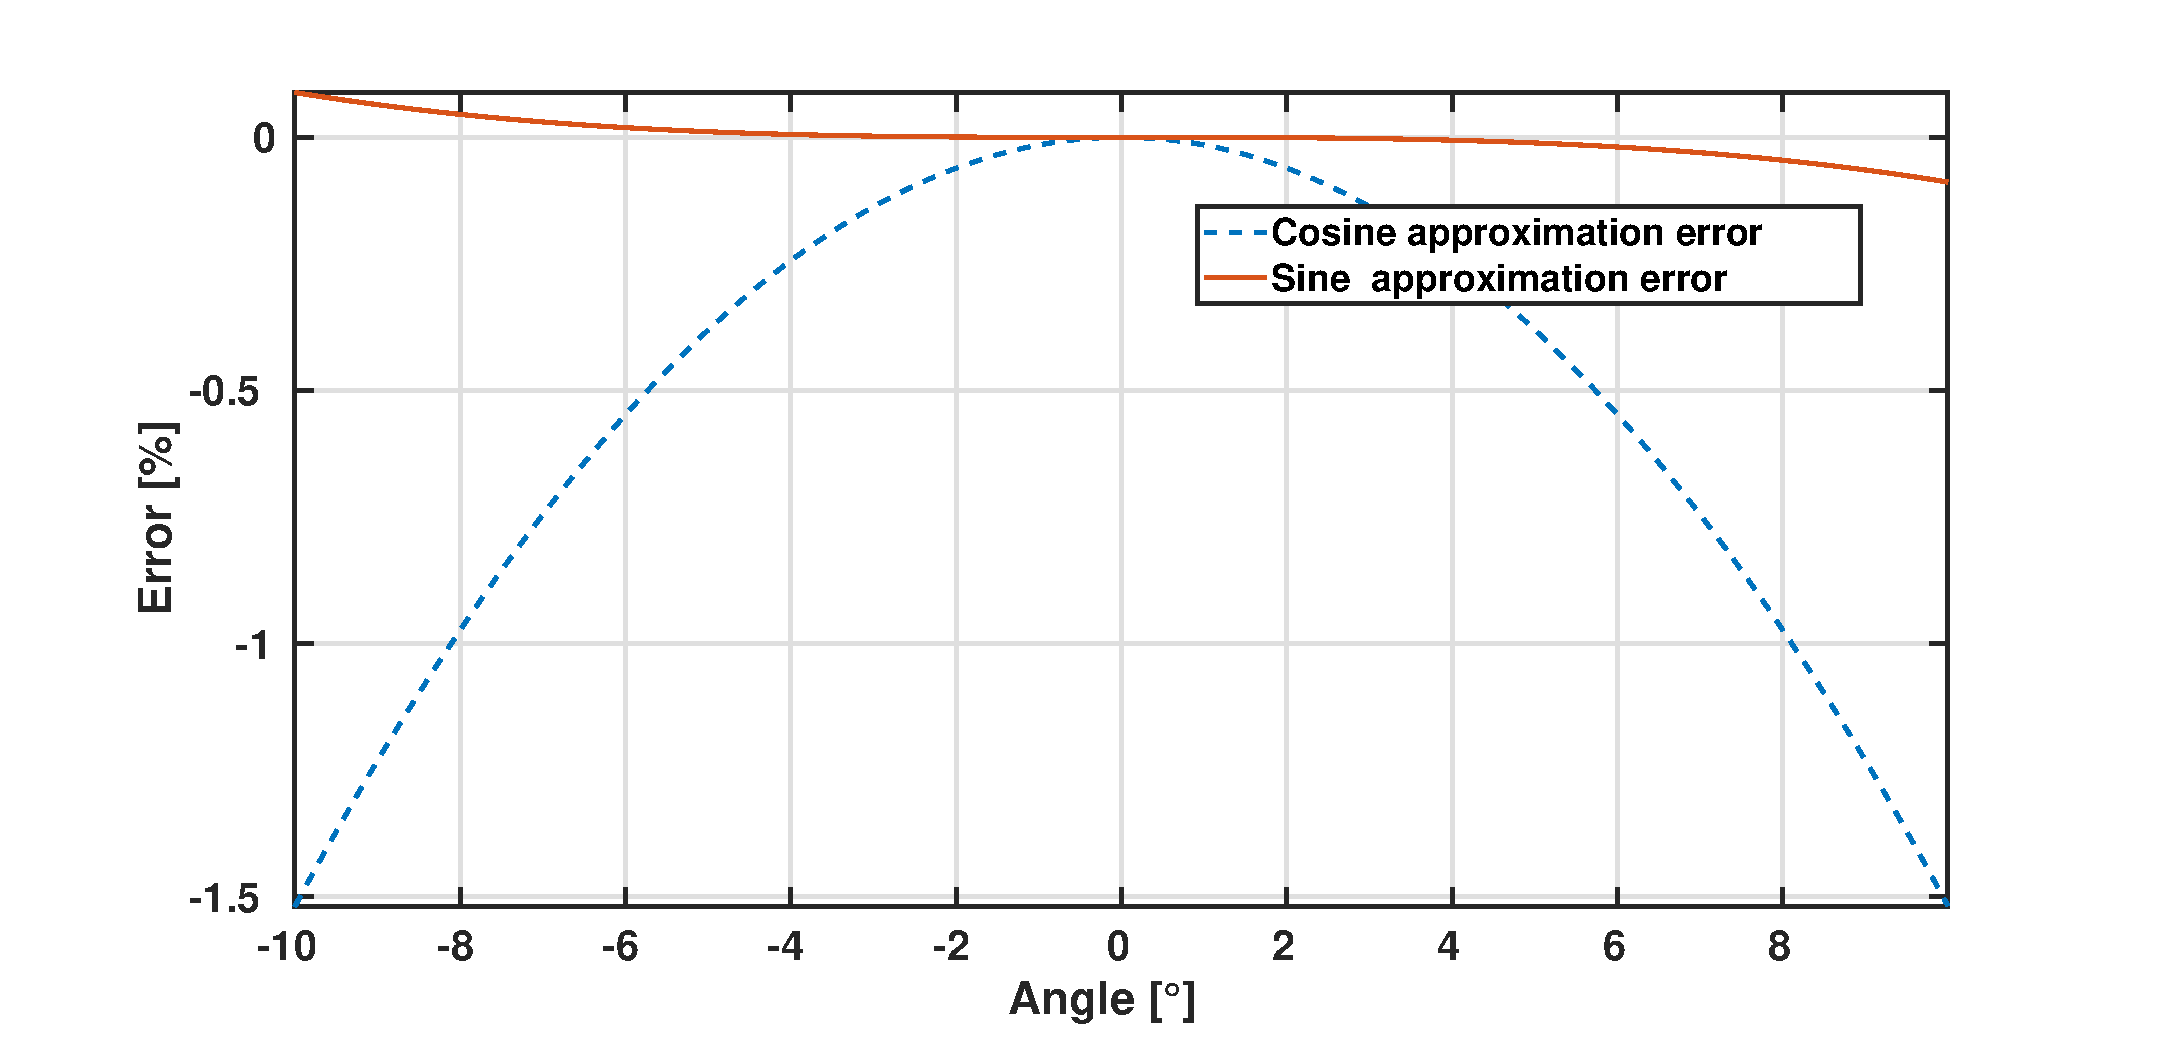
\includegraphics[width=0.8\textwidth]{CosSinLinApprox}
%	\caption{Error generated by the approximation of the cosine and the sine function}\label{fig:BasLinPlot}
%\end{figure}

